
Mais recentemente, \cite{Gladys2013} desenvolveram a
ferramenta \emph{User-driven Feature Space Transformation}
(UDFST) que possibilita ao usuário modificar os
atributos de um conjunto de dados com base na manipulação
sobre amostras dos itens. Neste trabalho os autores se
preocuparam em não sobrecarregar o usuário com interfaces  
demasiadamente complexas. Eles fazem uso de mapeamento de
elementos no plano para permitir interações mais intuitivas.


% Particularmente em aplicações de avaliação de funções
% multidimensionais~\cite{Jayaraman2002,Weber2007,Matkovic2008,
% Guo2009}. 

No contexto da indústria automotiva, \cite{Berger2011}
desenvolveram uma ferramenta para investigação de como as
decisões tomadas pelos projetistas afetam o desempenho dos
veículos produzidos, como o torque, a emissão de poluentes e
o consumo de combustível. Nesta aplicação o objetivo dos
usuários, no caso os projetistas, é definir os parâmetros de
modo a se obter um resultado ótimo. A ferramenta não é
restrita somente a este domínio, sendo aplicável em
qualquer contexto onde exista uma função e queira-se
verificar como os diferentes valores dos parâmetros 
afetam o resultado.

No entanto, como mostra a Figura~\ref{fig:berger}, os
mecanismos de interação propostos se baseiam em interfaces
que são demasiadamente complexas o que dificulta as
análises, principalmente quando o usuário lida com um grande
volume de dados.

\begin{figure}[h!]
    \centering
    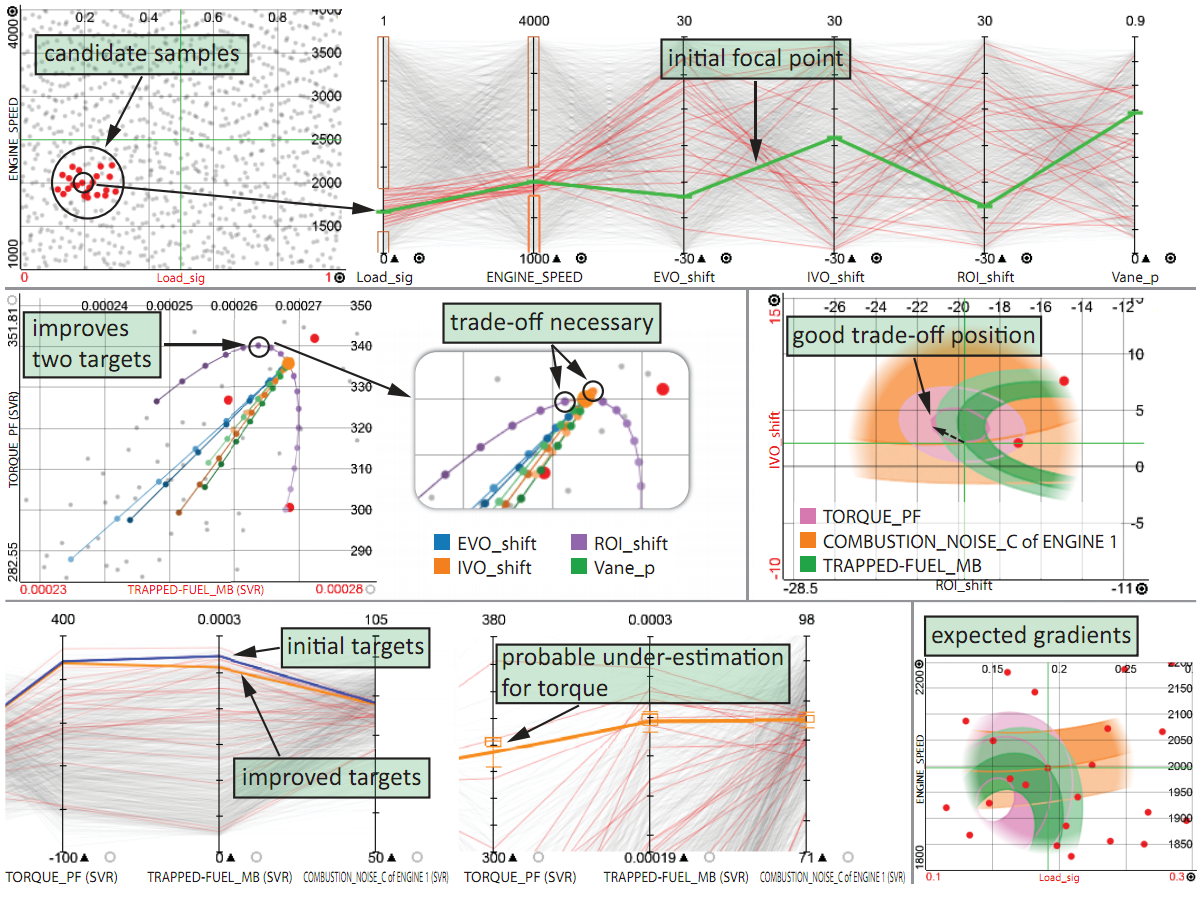
\includegraphics[width=16cm]{images/berger.png}
    \caption[Ferramenta proposta por \cite{Berger2011}]
    {Ferramenta proposta por \cite{Berger2011}. Mais do que detalhar cada janela, pretende-se ilustrar com
esta figura a complexidade da ferramenta. O usuário interage
com uma variedade de representações visuais, onde cada uma exige
um modo particular de análise.}
    \label{fig:berger}
\end{figure}

% Model space: avaliada somente em alguns poucos pontos de X.
% Externalising abstract: redução
% Interactive visual steering: scatter plots
% Uncertainty-aware: combinação em um único ambiente
% Topological landscapes: metáforas visuais e topologia
% A radial focus+contex: segmentação do espaço de parâmetros 


\subsection{VaR: Value and Relation}\label{sec:var}

Uma etapa fundamental da técnica Var que merece uma maior atenção é o método utilizado para a criação da matriz de distâncias. Os autores desenvolveram um novo método para cálculo da correlação entre dimensões que busca encontrar a maior discriminação entre os atributos. A seguir apresenta-se uma breve  descrição deste método:

\begin{enumerate}
   
    \item Dado um conjunto de dados com $m$ dimensões; 
    \item Normaliza-se os valores em respeito às colunas (invariância contra escala e translação);
    \item Para cada par de dimensões $Par(i,j)$ com $1 \leq i \leq m$ e $i < j \leq m$, constrói-se um histograma da diferença entre os valores $Hist(i,j)$. O número de \emph{bins} (classes) do histograma $numBins$ é uma constante definida pelo usuário;
    \item Para $k = 1$ até $numBins$ calcula-se $Var_k$:
    \begin{enumerate}
        \item Constrói-se a matriz $M_k$. A posição $M_k(i,j)$ da matriz será dada pelo valor $1$ subtraído da razão entre a população contida em $k-$classes mais frequentes de $Hist(i,j)$ e o total de elementos;
        \item $Var_k$ corresponde à variância dos elementos não diagonais da matriz;
    \end{enumerate}
\item Retorna-se $M_k$ que apresenta maior $Var_k$.

\end{enumerate}

Este método foi comparado à distância euclidiana entre os elementos e mostrou-se que o novo método apresenta um aumento na discriminação entre os atributos de $45\%$ a $95\%$ maior. Ou seja, utilizando este método, os autores conseguiram separar melhor dimensões diferentes e agrupar melhor as que apresentam certa semelhança. No entanto, não foram realizadas comparações com outras medidas de correlação entre variáveis bem estabelecidas na  literatura (para uma melhor discussão sobre essas medidas favor consultar a Subseção~\ref{ss:sim}). Apesar dos autores mencionarem que o cálculo de uma medida de correlação não está vinculado ao processo da técnica de visualização, trata-se de uma etapa diretamente relacionada com a projeção dos dados, consequentemente está fortemente atrelada à qualidade do \emph{layout} apresentado.

\subsection{Corrgram e  Coord}

Coord aborda o problema de que subconjuntos dos dados podem apresentar características diferentes, assim em alguns casos é impossível encontrar um único conjunto de atributos que represente todos os subconjuntos adequadamente. 

Quando o número de dimensões está na casa das centenas ou dezenas, não é possível inspecionar todas as dimensões exaustivamente. Assim, métodos estatísticos são utilizados para fornecer medidas de comparação entre os atributos. Entre essas medidas, as mais utilizadas são medidas de correlação estatística.

Medidas de correlação são normalmente apresentadas com o auxílio de uma matriz de correlação~\cite{Friendly2002}. Este tipo de representação é útil para se ter uma visão geral das relações entre pares de elementos e permite que um grande número de itens seja analisado. No entanto, para análises mais detalhadas, ou que exijam uma comparação entre mais do que simplesmente pares de elementos, não é uma representação adequada.

\subsection{RBF}

\citeauthor{Shneiderman2004} desenvolveram o framework Rank-by-Feature~\cite{Shneiderman2004} com o intuito de auxiliar a descoberta de correlações entre atributos. Eles classificam os atributos com base em critérios estatísticos definidos pelo usuário e possibilitam a construção de projeções uni ou bidimensionais para a avaliação da classificação realizada. 

Certas análises podem exigir demasiado esforço do usuário, devido à necessidade de se explorar individualmente cada dimensão ou avaliar par a par as relações entre atributos. Com a ocorrência de dependências não lineares este problema torna-se ainda maior e o usuário pode facilmente se perder em suas análises e não extrair novos conhecimentos dos resultados.

\subsection{Smart stripes e Guiding}

\cite{May2011} parte da ideia introduzida em \cite{May2011ss} para propor uma técnica para avaliação e orientação do processo de feature selection com base em métodos interativos visuais. Trata o problema de que diferentes partições das entidades dos dados podem apresentar  importâncias distintas de features. Permite que o usuário participe do processo de seleção e a investigue as dependências e interdependências entre conjuntos de features e itens.

Um problema desta técnica é a necessidade de se estabelecer uma feature de referência, pois a representação visual apresenta apenas as relações de 1-n.

\subsection{PCA, MDS e SOM}


Existem três principais abordagens para se reduzir a dimensionalidade dos conjuntos de dados a partir da combinação dos atributos. Análise de Componentes Principais (\textit{Principal Component Analysis)}~ ou simplesmente PCA, realiza combinações lineares sobre os atributos de modo que o novo espaço agregue a maior parte da variância dos dados. Para análises onde relações não lineares devem ser consideradas, \textit{Multimensional Scaling} (MDS) é uma alternativa interessante, pois trata-se de um algoritmo de otimização iterativo não linear, que busca minimizar as distâncias entre os elementos no espaço projeto e no espaço original. A área de aprendizado de máquina contribuiu com o método não supervisionado \textit{Self Organizing Maps} (SOM) para transformar conjuntos de dados em mapas bidimensionais.

% PCA methods can only work well for linear relationships.

% MDS e SOM: The impact of every original dimension is more or less still there.

% Scalability to high dimensionality. Although efficient algorithms for K-means or EM-based clustering have been developed repeatedly using such clustering algorithms to evaluate a large number of candidates (i.e., subsets of dimensions) can still cause computational efficiency problems, especially when both d and n are large.

Ao lidar com dados de alta dimensionalidade, costuma-se preceder a visualização com métodos ``caixa-preta'' como \textit{Principal Component Analysis} (PCA)~\cite{Wold1987},  \textit{Multimensional Scaling} (MDS)~\cite{Mead1992} ou \textit{Self Organizing Maps} (SOM)~\cite{Kohonen1990}. Apesar de popular, esta abordagem não utiliza os conceitos da área de visualização ao seu favor, pois o usuário não participa na etapa crucial da geração dos resultados, a redução de dimensionalidade.

PCA is not effective in identifying relationships or patterns that reside in different subspaces. SOM uses measurements from all original dimensions to derive the projection to a 2-D space and therefore noisy or irrelevant dimensions have dramatic impacts on the projection result

\subsection{iPCA}

Existem trabalhos que buscam contornar esse problema ao incluir a participação do usuário nesses métodos e tornar essas ``caixas pretas'' mais compreensivas. A técnica iPCA~\cite{Jeong2009}, por exemplo, provém meios para o usuário manipular os parâmetros da técnica PCA e, assim, ser capaz de entender mais facilmente as transformações realizadas sobre os dados. Similarmente, MDSteer [24] permite que o usuário guie o processo de MDS ao escolher regiões de interesse para se concentrar os esforços computacionais. No entanto, os mecanismos de interação propostos por esses trabalhos se baseiam em interfaces que são demasiadamente complexas ou que não contém todos os mecanismos necessários para lidar com um grande volume de dados.

Métodos mais sofisticados têm sido desenvolvidos para lidar com as novas exigências impostas pelos grandes conjuntos de dados e que se preocupam em fornecer interfaces intuitivas aos usuários. Estes métodos combinam diversas técnicas em um sistema integrado e possibilitam a interação do usuário para viabilizar a exploração de conjuntos de dados que possuem um elevado número de atributos.
